\section{Kiến trúc công cụ}

\begin{figure}[H]
	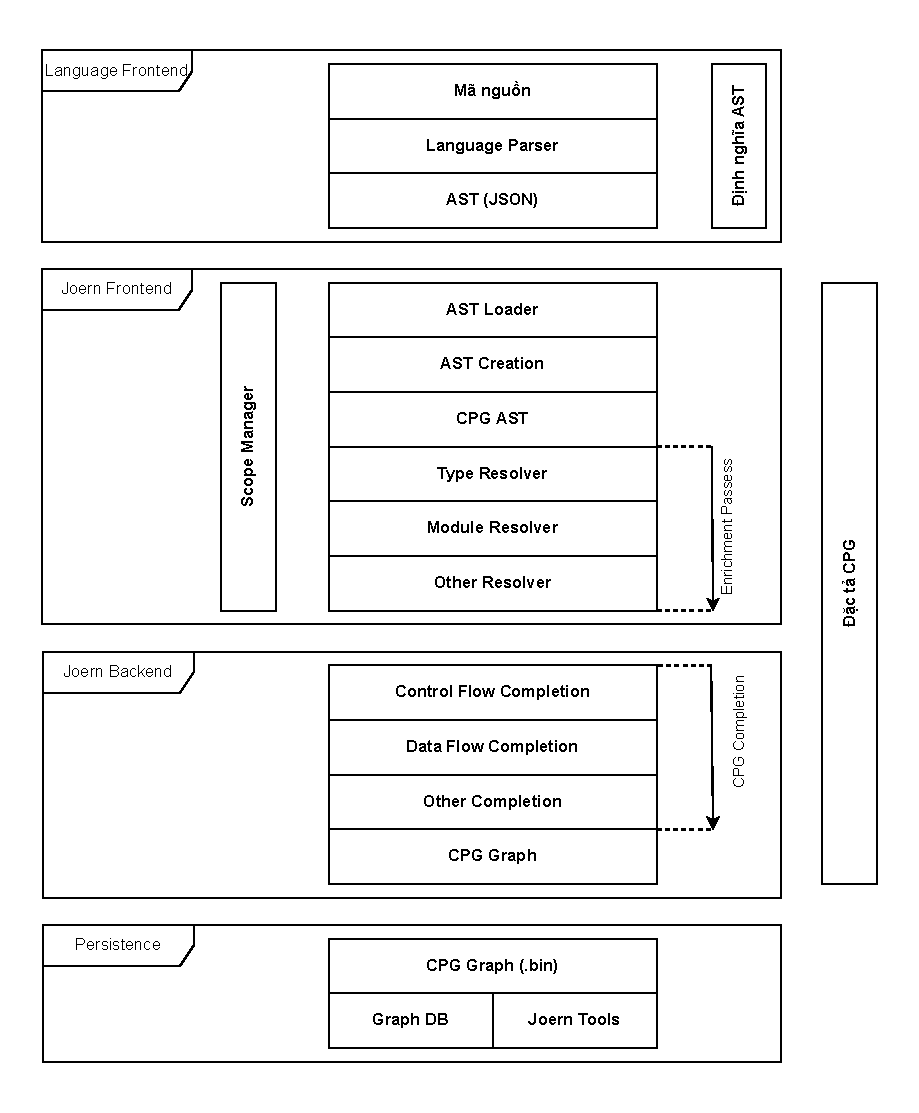
\includegraphics[width=1\columnwidth]{figures/c3/c3_arch.drawio.pdf}
	\centering
	\caption{Kiến trúc công cụ.}
	\label{img:c3_arch}
\end{figure}

Kiến trúc của công cụ về cơ bản sẽ là kiến trúc của Joern và mở rộng thêm.
Phần này sẽ đi chi tiết hơn so với phần \ref{sec:joern_flow} đã trình bày ở phía trên.
Các thành phần kiến trúc của công cụ bao gồm:

\textbf{Language Frontend.} Đây là phần đặc thù của mỗi ngôn ngữ lập trình, người dùng cần tự đảm nhiệm phần này khi muốn mở rộng ngôn ngữ lập trình mới cho công cụ Joern.
Nhiệm vụ của Language Frontend là chuyển đổi mã nguồn thành cây AST dựa trên định nghĩa AST của đặc tả ngôn ngữ.
Language Frontend có thể được cài đặt bằng bất cứ ngôn ngữ nào, do đó để có thể chuyển tiếp dữ liệu cho quá trình tiếp theo, Language Frontend cần xuất cây AST ra một loại dữ liệu trung gian, ở đây là JSON.

\textbf{Joern Frontend.} Là nơi chính thực hiện các công việc chuyển đổi cây AST của một ngôn ngữ lập trình thành cây CPG theo đặc tả CPG.
Đặc tả CPG sẽ được sử dụng xuyên suốt bởi Joern Frontend và Joern Backend.
Joern Frontend sẽ nhận dữ liệu từ Language Frontend dưới dạng JSON bằng AST Loader.
Cây AST sau khi được nạp vào Joern Frontend dưới ngôn ngữ Scala thì sẽ được chuyển đổi thành cây CPG bởi AST Creation.
AST Creation thực hiện ánh xạ mỗi một loại nút AST của ngôn ngữ sang một loại nút CPG tương ứng.
AST Creation còn tạo các cạnh giữa các nút, giữa các nút có thể có nhiều cạnh, mỗi cạnh thể hiện một mối quan hệ giữa các nút.
Mặc định giữa các nút có mối quan hệ là cạnh \texttt{AST}.
Tùy vào thể loại nút thì sẽ có các cạnh thể hiện mối quan hệ khác, ví dụ nút \texttt{IF} sẽ có cạnh \texttt{CONDITION} nối với nút thể hiện biểu thức điều kiện.

\textbf{Scope Manager.} Được sử dụng trong Joern Frontend để thực hiện quản lý phạm vi của các biến, hàm hay các khai báo khác.
Trong phần lớn các ngôn ngữ, một đơn vị thành phần sẽ có định danh riêng và định danh đó chỉ hợp lệ trong một giới hạn nhất định.
Trong quá trình duyệt cây AST, Scope Manager sẽ kiểm soát thông tin về các định danh và phạm vi hoạt động của chúng.
Khi sử dụng một định danh hoặc khai báo một định danh mới, Scope Manager sẽ kiểm tra xem khai báo đó có hợp lệ trong phạm vi hay không.
Với Scope Manager ta có thể xác định được quan hệ giữa việc khai báo và sử dụng một biến, hàm hay đơn vị cấu trúc khác, từ đó có thể xác định được các cạnh giữa các nút trong cây CPG.
Các cạnh sau này sẽ được sử dụng để xây dựng đồ thị CFG và đồ thị PDG.

\textbf{Passes.} Một phần của cây CPG bao gồm các nút và cạnh đã được xây dựng ở AST Creation kết hợp với Scope Manager.
Sau đó cây CPG sẽ tiếp tục được làm giàu thông tin bằng cách đi qua các pass.
Mỗi pass sẽ bổ sung một lớp thông tin riêng biệt, ví dụ thông tin về kiểu dữ liệu, cấu trúc module, thứ tự thực hiện câu lệnh, ...
Các lớp thông tin này hoàn toàn phụ thuộc vào ngữ cảnh của ngôn ngữ, do vậy số lượng pass cũng sẽ không cố định.
Các pass thao tác trên cây CPG nên có thể dùng chung cho nhiều ngôn ngữ, nhưng cũng có các pass được xây dựng riêng cho đặc điểm của một ngôn ngữ cụ thể.
Một pass có thể phụ thuộc vào kết quả của pass trước đó hoặc chạy độc lập nên thứ tự chạy các pass cũng rất quan trọng.
Ở đây, công cụ chỉ sử dụng 2 pass là Type Resolver và Module Resolver để xử lý hệ thống kiểu và hệ thống module của Rust, các pass khác sẽ được xây dựng trong tương lai.
Sau khi chạy qua các pass, cây CPG đã được bổ sung các lớp thông tin nhất định và đây cũng là công đoạn cuối cùng của Joern Frontend.

\textbf{Joern Backend.} Khi chuyển đổi một ngôn ngữ sang đồ thị CPG, người dùng phải tự thực hiện công đoạn Language Frontend và Joern Frontend để xây dựng cây CPG.
Các thông tin có được từ 2 bước trên sẽ được Joern Backend tận dụng để tự động hoàn thiện cây CPG thành đồ thị CPG.
Các nút, cạnh mới về luồng điều khiển, luồng dữ liệu sẽ được thêm vào và kết nối với các cạnh, nút đã tồn tại.
Không chỉ lớp thông tin về điều khiển và dữ liệu, Joern Backend bổ sung các lớp thông tin như  \texttt{FileSystem}, \texttt{CallGraph}, \texttt{Shortcuts}, \texttt{TagsAndLocation}, \texttt{Annotation} \cite{joernCodeProperty}.
Kết quả cuối cùng của Joern Backend là một đồ thị CPG hoàn chỉnh.

\textbf{Persistence.} Đồ thị CPG có thể được lưu trữ bền vững dưới dạng tệp nhị phân.
Tệp này có thể tiếp tục được chuyển đổi thành kiểu dữ liệu tương thích với các cơ sở dữ liệu đồ thị như Neo4j để thực hiện các truy vấn phức tạp, hoặc sử dụng với các công cụ khác của Joern.
